\documentclass[11pt, a4paper, leqno]{article}
\usepackage{a4wide}
\usepackage[T1]{fontenc}
\usepackage[utf8]{inputenc}
\usepackage{float, afterpage, rotating, graphicx}
\usepackage{epstopdf}
\usepackage{longtable, booktabs, tabularx}
\usepackage{fancyvrb, moreverb, relsize}
\usepackage{eurosym, calc}
% \usepackage{chngcntr}
\usepackage{amsmath, amssymb, amsfonts, amsthm, bm}
\usepackage{caption}
\usepackage{mdwlist}
\usepackage{xfrac}
\usepackage{setspace}
\usepackage{xcolor}
\usepackage{subcaption}
\usepackage{minibox}
% \usepackage{pdf14} % Enable for Manuscriptcentral -- can't handle pdf 1.5
% \usepackage{endfloat} % Enable to move tables / figures to the end. Useful for some submissions.


\usepackage[
    natbib=true,
    bibencoding=inputenc,
    bibstyle=authoryear-ibid,
    citestyle=authoryear-comp,
    maxcitenames=3,
    maxbibnames=10,
    useprefix=false,
    sortcites=true,
    backend=biber
]{biblatex}
\AtBeginDocument{\toggletrue{blx@useprefix}}
\AtBeginBibliography{\togglefalse{blx@useprefix}}
\setlength{\bibitemsep}{1.5ex}
\addbibresource{refs.bib}





\usepackage[unicode=true]{hyperref}
\hypersetup{
    colorlinks=true,
    linkcolor=black,
    anchorcolor=black,
    citecolor=black,
    filecolor=black,
    menucolor=black,
    runcolor=black,
    urlcolor=black
}


\widowpenalty=10000
\clubpenalty=10000

\setlength{\parskip}{1ex}
\setlength{\parindent}{0ex}
\setstretch{1.5}


\begin{document}

\title{Skills and Wages\thanks{Poooja Bansal, University of Bonn. Email: \href{mailto:pooja.bansal2610@gmail.com}{\nolinkurl{pooja [dot] bansal2610 [at] gmail [dot] com}}.}}

\author{Poooja Bansal}

\date{
{\bf Preliminary -- please do not quote} 
\\[1ex] 
\today
}

\maketitle


\begin{abstract}
	We provide joint evidence on the relationship between individuals’ cognitive abilities, their personality and earnings for individuals in  Germany using Mincer approach. The paper also estimates the relationships for different categories of occupation defined using the Goldthorpe  classification, 1992. With the data from the German Socio-Economic Panel Study, we employ scores from two short IQ-tests and a set of measures of personality traits which includes items from the Five Factor Personality Inventory. We regress our variables on log hourly wages using different specifications. The results suggest Education and experience are significant factors in the labor market. Our estimates for cognitive abilities indicate no association with wages for any occupations whereas for personality traits, our findings are heterogeneous, varying for different occupations.\\
\\
Keywords: Cognitive skills, Personality traits,SOEP, Occupation, Mincer, Wages \\
\\
Acknowledgement:  We would like to thank Prof.Dr.Thomas Dohmen and Dr.Philipp  Eisenhauer, University of Bonn for providing us with their expertise and guidance during the course of this research.
\end{abstract}
\clearpage

\section{Introduction} % (fold)
\label{sec:introduction}

There has been a growing interest in understanding the effects of non-cognitive skills and personality traits, on labour market outcomes. Many empirical studies have recognized the increasing importance of non-cognitive skills along with the cognitive skills. We try to build on this by studying the effects of both cognitive and non-cognitive skills on individuals’ wage profiles. Since the requirements for these skills vary with different occupations, we investigate the variations  by analyzing how these skills affect the wage profiles of individuals across different occupation levels.\par
The objective of this paper is twofold. We first examine whether cognitive and non-cognitive skills explain difference in hourly wages after controlling for experience and schooling, particularly the relative magnitude of the impact. Secondly we seek to estimate how the skill demands vary across different occupation levels. \par

People typically embody both type of skills: Cognitive skills driving their reasoning and thinking; and non-cognitive skills incorporating their personality traits.
Neisser (1996) defines Cognitive skill as “the ability to understand complex ideas, to adapt effectively to the environment, to learn from experience, to engage in various forms of reasoning, to overcome obstacles by taking thought.” There are numerous studies that have established measurements for cognitive abilities, for instance AFQT scores derived from the Armed Services Vocational Aptitude Battery (ASVAB) , GAT scores test which exists in the Commonwealth nations and IQ performance tests by DIW, Germany. These scores usually approximate cognitive abilities.\par
Most of the literature so far has focused on cognitive abilities only and ignored the importance of non-cognitive skills in labour market analysis due the fallibility of the measures. The skills, popularly known as the personality traits, encompasses many abilities perseverance, patience, reliability, cooperation, emotional stability, self-efficacy, self-esteem and security. Many economists have produced large body of evidence that employers in labor market have recognized the relationship between non-cognitive skills and productivity. This recognition have led to the evolution of measures like  Rosenberg Self esteem scale and Rotter Locus of control, the Big Five Factor Model to study the importance of these in the labor market. \par
The studies so far have discussed the importance of these skills in the labor market. We are contributing to this literature by establishing the relationships between these skills and occupations. But to what extent is occupation useful to understand how education and skills are related with wages. With the rapidly changing trends in the global labor market, employers today want their employees to possess a certain degree of qualification, in terms of skills, education and experience, due to the  non-pecuniary characteristics of different jobs. And in this highly competitive market, employees are keen to develop their qualifications to suit the market needs. Hence we see how these qualifications change in the occupational hierarchy.

This paper continues in the following order: In the next section we will discuss some of the literature which focuses on similar research area that helped us structure our expectations. In the Data section, we describe our data and source. In the Methodology section, we present our econometric framework, followed by the Result section where the first part explains the general relationship of skills for different individuals and then in the second part, we explore the differences in the relationships across various occupational levels. We then provide the robustness checks and finally conclude our analysis.

\section*{Literature Review}

There have been numerous studies which investigated the effect of cognitive skills and personality traits on wages.Heineck and Anger (2008) confirms that employers highly value individuals’ skills. Farkas (1997), Jenkins (2001) also confirm that employers assess cognitive and non-cognitive skills for hiring, promotion and wage setting policies.\par

On one hand, some studies suggested substantial returns to cognitive skills Anger \& Guido Heineck (2005) have established a positive relationship between cognitive skills and labor market outcomes, suggesting that abilities are correlated to the
wages in a significantly positive way for German workers.Murnane, Willett \& Levy (1995) also recognized the importance of cognitive skills in wage determination.While on the other hand, many research works found that cognitive ability has a very little  or no effect on earnings.(Bound et al.(1986)). Also, Cawley, Heckman \& Vytlacil (2001) and  Zax \& Rees (2002) reported that the effect of cognitive skills is much smaller than what has been asserted by previous analyses and is rather a poor estimator of earnings.\par

As for personality traits, attention is growing towards its relationship with labor market. Gintis \& Osborne( 2001) explained how some personality traits matter for employers because they facilitate the production of effort at work and affect labour productivity. 
Heckman,Stixrud \& Urzua (2006) suggested that non-cognitive skill is an equally strong determinant, if not more, as cognitive skill. Bowles \& Gintis (1976) and Edwards (1976) in their work showed that skills such as dependability and persistence are highly valued by employers.\par

However, studies have not sufficiently recognised the role that occupation plays, along with the individuals' skills, in the determination of wages. Beyer\& Knight(1989) studied how wages vary across different occupations in Africa. Birnbaum (1976) interpreted the observed effect of a worker's initial skill category on his current wage. Stewart (1977) found that the British returns to education were generally higher in the non-manual than in the manual occupations and lowest for the unskilled, and that the returns to experience also differed considerably by occupation. Carbonaro (2007) explained that education and cognitive skills are positively related to earnings among workers within narrowly defined occupations.

Overall there is vast literature on the importance of both kinds of skills for wage determination. With our paper, we take a closer look at the wage-skill relationships across different occupational levels.


\section*{Expectations}

With the prior findings from previous empirical studies on non-cognitive and cognitive skills as determinants of labor market outcomes, we were able to set up expectations for the present study. 
In line with the previous research, we expect cognitive skills to have either positive or no association with the earnings. With respect to the personality traits used, we expect no significant relation between Extraversion and wages, a positive relationship for Openness and conscientiousness and negative for Neuroticism and Agreeableness.\par

We believe we are the first one to investigate this skill-wage relationship with respect to occupations using the Goldthorpe classification. So we built our expectations based on our knowledge of the subject.For occupations, we expect cognitive skills to be either positively or not related to the occupational categories. For personality traits, we expect more heterogeneous results for each category of occupation, depending on their work task and roles.


\section*{Data}

This paper analyzes the data from the German Socio Economic Panel. SOEP is a wide-ranging representative micro-database providing comprehensive socio-economic information on private households in Germany. The panel was first started in 1984 and data for about 12,200 randomly selected respondents, in West Germany, was collected. After German reunification, data for about 4500 respondents, from East Germany, has been added. We use two recent waves which include data on cognitive skills (2005), two short verbal and performance tests, and personality traits (2006), items pertaining to the Big Five Factor model. We retrieved the data for occupation and education from the personal questionnaire of 2005. 

\subsection*{\textit{\underline{Measures of Cognitive skills}}}
The fully fledged IQ tests couldn’t be conducted because of the large scale panel survey.The organization conducted two short tests to evaluate cognitive skills in year 2006. These were: A Word Fluency Test and Symbol Correspondence Test. These tests correspond to modules  of the Wechsler Adult Intelligence Scale (WAIS)\footnote{Wechsler Adult Intelligence Scale (WAIS) comprises 14 modules, seven on verbal IQ and seven on performance IQ (Groth-Marnat, 1997, Kline, 1999)}. 
For the Word Fluency test, which corresponds to the verbal IQ module of WAIS, respondents were asked to name as many animals as possible in 90 seconds and for the Symbol Recognition Test, corresponding to the Performance IQ module, respondents had to match as many number and symbols as possible in 90 seconds using the correspondence list provided to them. We have standardized the test scores since they were measured on different scales.

\subsection*{\textit{\underline{Measures of Non-Cognitive skills}}}

Over time, psychologists have developed a widely accepted personality taxonomy known as the Big Five model which identifies five broad aspects of Personality namely: Openness, Conscientiousness, Extraversion, Agreeableness, and Neuroticism 
(OCEAN). Openness can be defined as a tendency to experience new adventures and emotions, to develop unusual ideas, and to have curiosity. Conscientiousness can be seen as a desire to act in an organized, disciplined, and dutiful manners. Aiming for organized planning instead of spontaneous behaviours. Extraversion can be associated with optimistic behaviours and positive energy, where a person tends to seek attention and interaction in the company of others. Agreeableness can measure if a person is well tempered and cooperative or if he/she is suspicious or untrustworthy. Neuroticism defines the level of emotional stability of a person and can be related to unpleasant emotions such as depression, anger or vulnerability. \par
In 2005, SOEP included questions related to individuals’ personality. The questions are associated to the Big Five Factor model which comprises of the personality aspects described above. Since extensive questioning to generate the scores pertaining to Personality wasn’t feasible in SOEP, the data instead provides us with 15 items\footnote{The items included and the classification is presented in the Appendix Table 1} in which three items apprehends to one personality dimension. The questions were answered on a scale of 1[does not apply] to 7[applies fully]. We have taken averages of the each three items of the respective personality factor of the big five model and standardized them. 

\subsection*{\textit{\underline{Determination of Hourly Wages }}}

SOEP doesn’t collect data on hourly wages directly. Instead it provides data on monthly income from primary employment and actual weekly working hours including overtime. We calculate the hourly wages by dividing the monthly income with the product of weekly hours and the estimated factor of 4.3\footnote{Number of weeks/Number of months = 52/12 = 4.3} for the number of weeks. The measurement errors, possibly existing in working hours or monthly income can influence the results. 

\subsection*{\textit{\underline{Analytical Sample}}}

To address the research question posted in the study, the analytical sample is limited to individuals between age 20 and 60  who were in full time employment, in order to include only those who most likely have completed their education and were below the retirement age. We excluded the observations which had missing values. For individuals reporting zero wages, a small value of 0.0001 was assigned before it was transformed to a logarithmic scale. For categorizing the occupations, we used the  Goldthorpe \footnote{ Goldthorpe class scheme combining occupation categories in light of level of income, economic security, advancement, work authority and responsibility.  
} classification scale.  We have, however,  excluded the category for  agricultural workers and self-employed people due to their very small sample size. The total sample size turned out to be 2581\footnote{The sample size in our analysis rather low since we had to restrict our sample to the  individuals who are SOEP respondents in both 2005 and 2006 and, more limiting, were the CAPI surveyed in 2006 for cognitive skills, since only those were the only potential respondents of the ultra-short IQ-tests.Further, for occupational classification we used the data from the generated variable file which led to a further reduction.}


\begin{figure}
    \caption{Frequency Distribution of Occupation}
    
    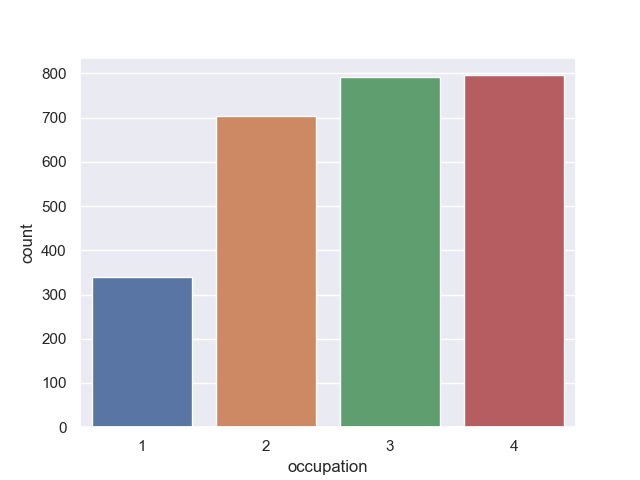
\includegraphics[width=\textwidth]{../../out/figures/occupation_count}

\end{figure}

\begin{figure}
    \caption{Correlation heatmap}
    
    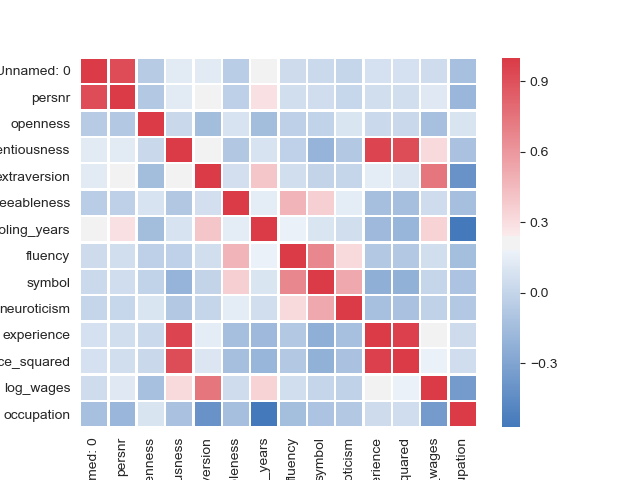
\includegraphics[width=\textwidth]{../../out/figures/heatmap}

\end{figure}

\begin{figure}
    \caption{Density plot for all the variables}
    
    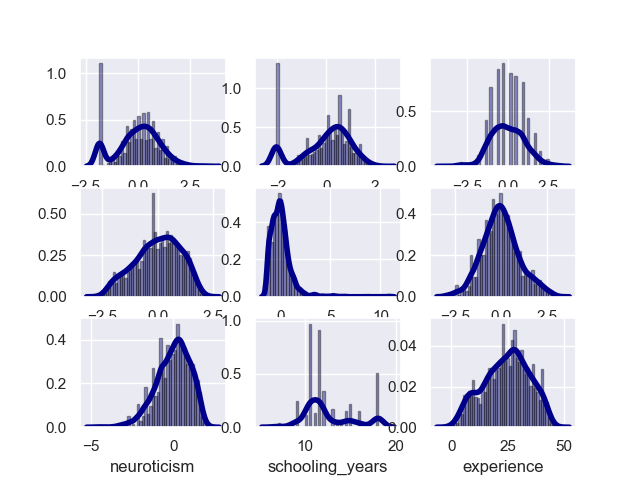
\includegraphics[width=\textwidth]{../../out/figures/distplot}

\end{figure}


\section*{Methodology}

First we investigate the returns to earnings by  using the basic Mincer\footnote{It was Jacob Mincer who in his book ‘Schooling,experience and earnings, 1975’ modelled log earnings as  the sum of linear years of schooling and a quadratic function of years of potential experience, experience being afe minus schooling minus six. The equation has been used by various researchers for estimation on a ton of data sets for a many countries and time periods which undeniably makes it one of the most widely used approach in empirical economics.} specification:
   \[lnY_{i} = \beta_{0} + \beta_{1}S_{i} + \beta_{2}E_{i} + \beta_{3}E^{2}+\epsilon_{i} \label{eq:basic} \tag{1} \]                        

Where lnY is the natural logarithm of hourly wages of individual i, S represents years of schooling and E is potential years of experience and E\textsuperscript{2} is squared experience.\par
There exists a linear relationship between schooling and wages.The variable experience is generated using the approach used in Johnson, Chow(1997)\footnote{Johnson,Chow in Rates of Returns to Schooling in China (1997) assume that the average person began his schooling at age  6  years  and  that  time  not  spent  in  formal  schooling  was  spent  gaining  on-the-job experience
}:
                     \[ Experience = Age- Schooling -6\]
                     
 A simplifying assumption of our model is that the cognitive skills are not correlated with education since the correlation can bias our results. The assumption is fair based on the evidence in Griliches \& Mason (1972)\footnote{Griliches and Mason, 1972 in Education,Income and Ability ( 972) investigated the contribution of education to economic growth and suggested that the mental ability is indeed correlated to the quantity of schooling since an individual obtains most of his mental ability in formal years of education which further contributes to his income.}
 We will then expand the basic specification by adding the cognitive skills to (1):
 \[lnY_{i} = \beta_{0} + \beta_{1}S_{i} + \beta_{2}E_{i} + \beta_{3}E_{i}^{2} + \gamma c'_{i} +\epsilon_{i} \label{eq:cog} \tag{2} \]  
 
 Here c' is the vector of individual i’s cognitive skills which includes the standardized test scores of Fluency and Symbol Recognition Test.
 We then introduce only non cognitive skills in the basic specification:
 
  \[lnY_{i} = \beta_{0} + \beta_{1}S_{i} + \beta_{2}E_{i} + \beta_{3}E_{i}^{2} + \alpha n'_{i} \label{eq:noncog}+\epsilon_{i} \tag{3} \]  
  
  n' is the vector of non cognitive skills which includes the standardized  five personality traits of the Five factor model. 
  
  We then add both skills to the specification (1): 
  \[lnY_{i} = \beta_{0} + \beta_{1}S_{i} + \beta_{2}E_{i} + \beta_{3}E_{i}^{2} + \gamma c'_{i} + \alpha n'_{i} +\epsilon_{i}  \label{eq:cog} \tag{4} \]
  
  We will then run regressions for the above mentioned specifications with respect to different occupations:
    
 \[lnY_{i,j} = \beta_{0} + \beta_{1}S_{i,j} + \beta_{2}E_{i,j} + \beta_{3}E_{i,j}^{2} + \gamma c'_{i,j} + \alpha n'_{i,j} +\epsilon_{i,j}  \label{eq:cog} \tag{5} \]
 
 Where lnY is now the log hourly wages of individual i with occupation j. 
 
 \section*{Results}
 This section presents estimates of the impact of cognitive and non-cognitive skills on the labor market outcomes. The first subsection presents estimates pf the relationship between skills and wages for  all the four describe specifications. The second subsection examines the impacts of those skills on wages across the occupation categories. 
% section introduction (end)

 \begin{table}[h!]
 \begin{tabular}{ |p{4cm}| p{2cm}| p{2cm}| p{2cm} |p{2cm}|  }
 \hline
 \multicolumn{5}{|c|}{\textbf{log wages}} \\
 \hline
  & (1) & (2)& (3)& (4)\\
 \hline
 & & & &\\
 Schooling Years   & 0.0732***   &0.0757***&   0.0694*** &0.0715***\\
  &(.0076) &(.0077)  &(.0077) &(.0078) \\
 Experience&   0.0749***   &0.0761***   &0.0731*** & 0.0745***\\
  &(.0088)  &(.0089) &(.0088) &(.0088)\\
 Experience squared & \textendash0.00115*** &\textendash0.00117*** &\textendash0.00113*** &\textendash0.00115***\\
  &(.00018) &(.00018) &(.00018) &(.00018)\\
 \textbf{Cognitive Skills} & & & &\\
 & & & &\\
 Fluency&   &\textendash0.0520&  &\textendash0.0497\\
 & &(.0284903) & &(.0283324)\\
 Symbol Recognition& &0.0173& &0.0246 \\
 & &(.0290053)& &(.028911)\\
 \textbf{Non-Cognitive Skills} & & & &\\
 & & & &\\
 Openness& & &\textendash0.0383 &\textendash0.0370\\
 & & &(.0225) &(.0225)\\
 Conscientiousness& & &0.0748*** &0.0723**\\
 & & &(.0220) &(.0220)\\
 Extraversion& & &0.0224 &0.0226\\
 & & &(.0224) &(.0224)\\
 Agreeableness& & &\textendash0.0989*** &\textendash0.0997***\\
 & & &(.0217) &(.0218)\\
 Neuroticism& & &\textendash0.101*** &\textendash0.101***\\
 & & &(.0210) &(.0210)\\
 & & & &\\
 \hline
\end{tabular}
\begin{flushleft}
{\footnotesize Standard error in parentheses\\
* p$<0$.05, ** p$<$0.01, *** p$<$0.001}
\end{flushleft}
\end{table}




Column 1 presents the estimates for variables in the the typical mincer equation. The point estimate of the schooling coefficient is 0.073 and highly statistically significant  which indicates that wages increase by around 7\% with an additional year of schooling. Experience is also statistically significant with an estimate of 0.074. \par
However, the ceteris paribus assumption does not work directly for experience since when we increase experience, experience squared increases as well. We therefore computed the partial effect. We found that with the average experience level of 24.23 years, there is a return of about 1.9\% per year of experience on average.\par
The results satisfy the findings by Mincer and various other economists. However, there has been a lot of criticism by economists for the Mincer Approach. Since we have already assumed there is no  correlation between skills and schooling, we have reduced the effect of the so called ability bias but the omitted variable bias is still persistent. There has been literature that suggests that there are other socio-economic factors affecting wages. The discussion regarding this is out of the scope of this paper. \par
Column 2 shows the estimates of the expanded Mincer equations using cognitive skills. The mincer estimates remain significant. As per our expectations, cognitive skills are found to be statistically insignificant. However, what is surprising is that the estimate for Fluency test scores shows negative association with wages. 
The insignificance of  test scores  and the negative association of the variables could be a result of various possible reasons. The Fluency test is possibly affected by measurement error since the interviewer had to instantly identify the duplicate answers given by the respondent which might have influenced our results. Also working memory of the individual comes into play due to the 90 second time constraint. Moreover, the data contains individuals with migration background who may not have sufficient language skills to respond as compared to the native speakers during the Fluency Test. \par
Column 3 shows the results for the addition of non-cognitive skills to the basic Mincer model. Substantially, the results show that some of our prior expectations are met while some are different from our hypothesis or previous findings.\par
As expected, there is no significant relationship between Extraversion and wages. The point estimate of 0.02 however indicates a positive relationship. 
For Openness, we particularly suggested a positive relationship with wages but the results show no significant association with a negative estimate of 0.038. In line with the expectations, Conscientiousness is highly statistically significant and has a positive association with wages. The point estimate of 0.074 suggests around 7\% wage premium for one standard deviation increase in Conscientiousness. \par
As per the expectations, Agreeableness is highly statistically significant and negatively associated with wages. The point estimate of 0.098 suggests the wage penalty of 10\% for ‘being nice’, i.e one standard deviation increase in Agreeableness. 
This, in general, however seems implausible in the first glance since we expect cooperative people to be preferred more by employers. But the agreeable individuals could be extremely cooperative in the sense that they might sacrifice their interests and careers by avoiding possible conflicts while trying to be nice. 
In line with the prior findings and our expectations, Neuroticism is negatively associated with wages and is highly statistically significant with the point estimate of 0.101. Thus, one standard deviation increase in Neuroticism results in 10\% wage penalty. \par
Column 4 shows the results for Mincer equation including all the cognitive and non-cognitive skills. We found that adding both the skills did not change the results much. The relationships tend to be the same with slight changes in the coefficients. 

\subsection*{\underline{Results with respect to  Occupation}}
We ran regressions for all the specifications mentioned above with respect to different occupational levels of Goldthorpe scale. The results tend to be the same for the final model including both kinds of skills and the individual models for the skills. We are discussing in details the results\footnote{The regression results for the other specifications with respect to occupations are given in Appendix Table 5} only for specification (5).  \par
For Higher  Managerial and Professional Workers (1), number of Schoolin years is no longer a significant variable but experience is still statistically significant.  This is possible because when one climbs the ladder of professional accomplishments, he gets to a step where the work experience overshadows the number of years she has spent on education.The cognitive skills are non significant with negative estimates as they were in the standard model. For the personality traits, Neuroticism and Agreeableness are the only significant skills. The sign of the other estimates are ,however, the same.  The point estimate of 0.18 for agreeableness suggests 18\% wage penalty for one standard deviation increase in Agreeableness while a standard deviation increase in Neuroticism results in 31\% wage penalty.\par

For Lower Managerial and Professional Workers(2), both Schooling years and experience are significant. This is plausible because these managers can still climb up the professional ladder for which both their education and work experience would matter. However, by the comparing the estimates,0.032 and 0.038, we can say that experience carries more weightage during such professional growth. Both the cognitive skill variables are again insignificant but the estimate for the symbol correspondence test is now positive. For personality traits, only Conscientiousness and Agreeableness matter for lower professional workers. The reason could be the same as previously mentioned. People aiming for higher managerial positions would have to show more efficiency and self-discipline and act dutifully. \par

For Workers in Routine Services(3),  the results for education and experience are the same as we had for basic specification. For this category of occupation, neither of the two skill sets are significant. For hiring the employees in this category, the employers would consider the experience and a certain level of education of the employees more than their other skill sets because they would be mostly in the administrative , commercial and sales activities where they require a particular skill set to perform a number of  routine tasks which do not have any technical aspects.\par

For the Manual Workers(4), the results for the variables in basic specification are in line with the standard results as expected since they would require the education, or say on-the job training, to perform the manual but skilled or semi-skilled tasks.Both Fluency Test and Symbol Correspondence test have significant relationship with wages. The reason could be that the people belonging in this occupation category, including plumbers, cooks, drivers, machinists etc, are on the lowest levels of occupational hierarchy , dealing directly with consumers, switching employers frequently and continuously improving and familiarizing themselves with the rapidly changing trends in equipment and consumer needs. As for the personality traits,   Neuroticism is the  only significant set of skills for Manual workers. \par

\begin{table}[h!]
\centering
 \begin{tabular}{ |p{4cm}| p{2cm}| p{2cm}| p{2cm}| p{2cm}|  }
 \hline
 \multicolumn{5}{|c|}{log wages} \\
 \hline
 Occupation & \textbf{1} & \textbf{2}& \textbf{3}& \textbf{4}\\
 \hline
 & & & &\\
 Schooling Years  &0.0170   &0.0321 * &0.0859***    &0.0520***\\
  & (0.0278)&(0.0146) &(0.0244)  &(0.0124) \\
 Experience& 0.0746*    & 0.0387* &0.109*** & 0.0546***\\
  &(0.0331 ) &(0.0173)  &(0.0191 ) &(0.0078) \\
 Experience squared & \textendash0.0009 &\textendash0.0004 &\textendash0.0018*** &\textendash0.0009***\\
  & (0.0007) &(0.00037) &(0.0004) &(0.0001) )\\
 \textbf{Cognitive Skills} & & & &\\
 & & & &\\
 Fluency&\textendash0.0201   &\textendash0.071 &\textendash0.0161 &\textendash0.0488*\\
 &(0.0962) &(0.0539) &(0.0630) &(0.0248) \\
 Symbol Recognition&\textendash0.0810 &0.0182&\textendash0.0161 &0.0587* \\
 & (0.0989)&(0.0550) &(0.0640)&(0.0258)\\
 \textbf{Non-Cognitive Skills} & & & &\\
 & & & &\\
 Openness&\textendash0.0346 &\textendash0.055 &\textendash0.06550 &\textendash0.01386\\
 &(0.0818) &(0.0427) &(0.0500) &(0.020)\\
 Conscientiousness&0.0325 &0.111** &0.0790 &0.0094 \\
 &(0.0825) &(0.0408) &(0.0475) &(0.0203)\\
 Extraversion&0.0335  &0.0513  &0.0259 &0.0057\\
 &(0.0730) &(0.0463) &(0.0498) &(0.0194) \\
 Agreeableness&\textendash0.1879* &\textendash.01051* &\textendash0.0687 &\textendash0.03155 \\
 &(0.0759) &(0.0420) &(0.0513) &(0.0191) \\
 Neuroticism&\textendash0.3158*** &\textendash0.0591 &\textendash0.0127 &\textendash0.0663***\\
 &(0.0713) &(0.0409) &(0.0474) &(0.0189)\\
 & & & &\\
 \hline
\end{tabular}
\begin{flushleft}
{\footnotesize Standard error in parentheses\\
* p$<0$.05, ** p$<$0.01, *** p$<$0.001}
\end{flushleft}
\end{table}

\section*{Robustness Checks}

We also ran additional regressions as robustness checks,since the results (Appendix Table 4) obtained are not much substantially different from those given above, we are not discussing them in detail. When we compared the averages for all the skill variables for both classes of gender, we observed that the figures vary significantly.  Also, due to differences in the pay scale for females and fluctuations in their professional career, there could be some possible bias in the results. Therefore, we first estimated our model for the male population only for which we got,more or less, the same results.However, a significant change in result was that Extraversion is now a significant trait.   \par
Also, the differences between people from different nationalities, in terms of their culture, upbringing and social behaviour, might have had an impact on the results. Hence,we restricted the data to individuals with German nationality only and again got results similar to our previous findings. 
The results for both the checks are given in Appendix Table 4. 

\section*{Conclusion}

In our paper, we provided the analysis of the relationship of wages with cognitive and non-cognitive abilities applying Mincer approach for individuals belonging to different occupations in Germany using SOEP data. \par
We first presented evidence that cognitive skills are not as good a determinant for wages as suggested by previous empirical works. Our results indicate that non-cognitive skills play the dominant role in explaining the labor market returns and differences among occupations.
We then explore these relationships for different occupational groups.\par
To sum it all up, the numbers of years spent on education is not relevant for individuals belonging to the higher level of occupational hierarchy but for those who are still aiming for higher positions in their professional career.\par
For all individuals, experience is positively associated, specially for lower managerial and professional workers.
Cognitive skills are not as strongly related to wages. As per our results, it is relevant only for a minor class, i.e. Manual workers, of working individuals.
Personality traits were, overall, significant except Extraversion which we expected. Neuroticism is significant for almost all individuals irrespective of the occupational category they belong to. Openness is negatively associated for all the individuals, surprising to our expectations. 
We used Mincer approach which is only one of many approaches followed by the economists. Also, there are some potential problems which have not been taken into account in this paper, like the possible endogeneous relationship between wages and personality which might result in reverse causality. The assumption made regarding the relationship between education and ability has been mathematically addressed by other studies. A further issue is the measurement error persistent in the measured skill variables which might have strongly affected the results. All these problems can be addressed using different approaches which have not been covered in the paper. 

\setstretch{1}
\printbibliography
\setstretch{1.5}




% \appendix

% The chngctr package is needed for the following lines.
% \counterwithin{table}{section}
% \counterwithin{figure}{section}

\end{document}
